\subsubsubsection{Scheduling}
The scheduling package contains all the logic needed to have static threads
which consume work items, which correspond to the actions that occur in our
simulations.

In Figure \ref{fig:schedule-workflow} we show how a request to schedule an
entity is handled:

\begin{enumerate}
  \item First, the \texttt{Scheduler} delegates the execution of an action to an
    \texttt{Executor}: the latter is an interface which is implemented by
    \texttt{SimpleExecutor} in our system;
  \item \texttt{SimpleExecutor} registrates a timer to defer the action;
  \item When the timer expires, it asks to its \texttt{Executor} reference to
    execute an action (the one which originally had to be scheduled);
  \item If it is not stopped, \texttt{SimpleExecutor} add this action to the
    \texttt{WorkQueue}
  \item and notifies the \texttt{CommandBroker} that there is new work;
  \item This causes the \texttt{CommandBroker} to open a guard and makes the
    \texttt{WorkerThread}(s) wake up;
  \item Each one of the \texttt{WorkerThread}s asks for item, consuming them
    until there is some.
\end{enumerate}

\begin{figure}[H]
\centering
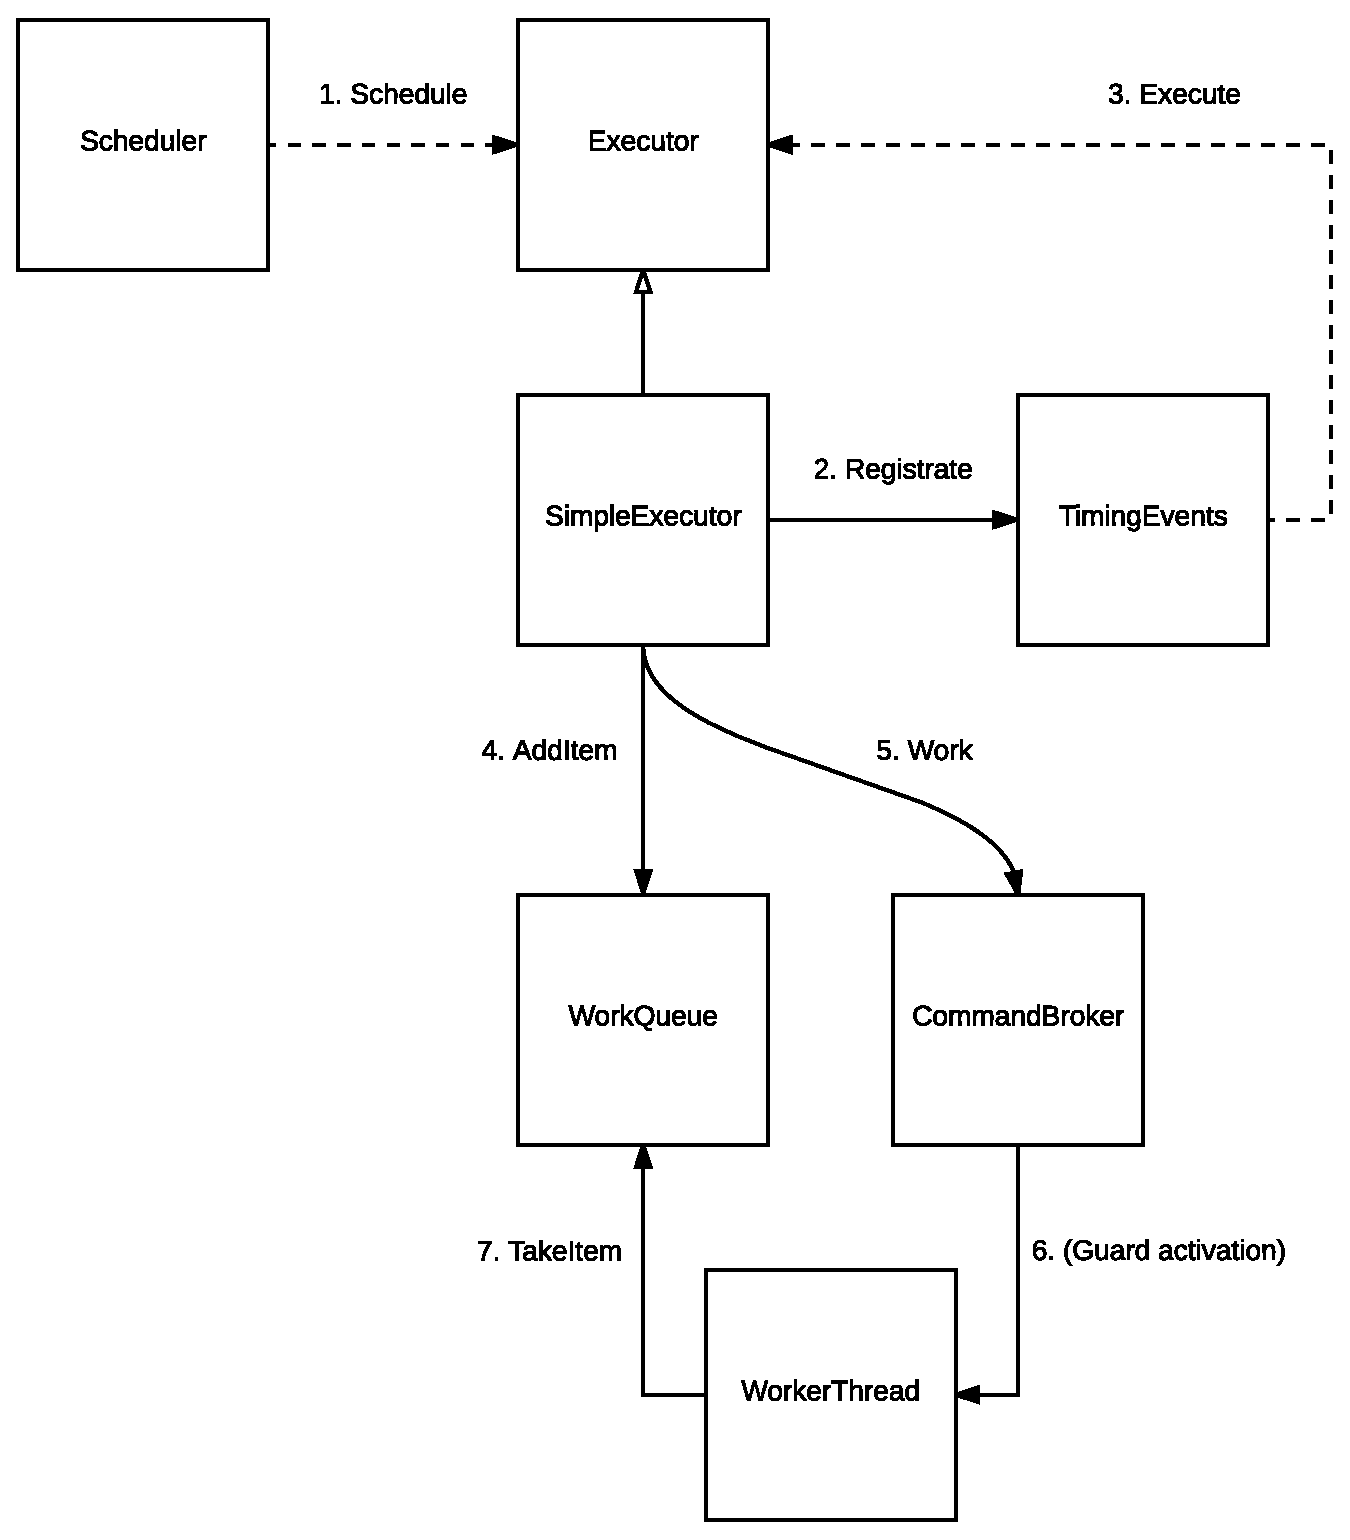
\includegraphics[scale=0.4,keepaspectratio]{images/solution/app/backend/scheduler.eps}
\caption{Schedule workflow}
\label{fig:schedule-workflow}
\end{figure}
